\chapter{\label{sec:sysCheck}Systematic uncertainties}
  In this chapter the methods used to estimate the systematic 
    uncertainties are described. 
  Table~\ref{tab:sumsyst} shows the systematic errors that were estimated.
  The method used to separate the coherent from the photon-photon process 
   is the most dominant uncertainty.
  This is followed by the systematic uncertainty on the integrated luminosity,
    which is discussed in \cite{cmsLumi}.
  The ZDC reconstruction method used to estimate the neutron thresholds 
    is the next most dominant, followed by the method used to estimate
    the HF noise threshold. 
  \begin{table}[!Hhtb]
    \begin{center}
      \begin{tabular}{|c|c|c|}
        \hline
        systematic & uncertainty in \%  \\ \hline
        Template fit normalization & +9.5\% -12.0\% \\ \hline
        Luminosity & 5\% \\ \hline
        ZDC trigger efficiency & 3.5\%    \\ \hline
        ZDC reconstruction  & 2.9\%  \\ \hline
        HF noise threshold & +1.3\% -3.4\% \\ \hline 
        MC acceptance & 1.1\% \\ \hline
        \hline \hline
        Total systematic & +12\% -14\% \\ \hline
      \end{tabular}
      \caption{Summary of systematic uncertainties}
      \label{tab:sumsyst}
    \end{center}
  \end{table}

  \section{Template fit normalization}
    The \pt{} template fit depends on the functions chosen for fitting
      the mass distribution.
    As described in Section~\ref{sec:sigEx}, the similarity of the 
      \pt{} distribution for the coherent and photon-photon process makes
      the contributions from the two process difficult to separate from the 
      \pt{} distribution alone.
    The mass distribution was used to distinguish between these two processes.

    The systematic uncertainty due to the choose of functions used to fit
      the mass distribution was estimated by varying the signal and 
      background functions.
    The contribution to the background from the mass fit was used to fix the
      contribution from the photon-photon process in the \pt{} template
      fit.
    Two functions were used to describe the signal, a Gaussian, and a Crystal
      ball function. 
    The background was fit to a linear function, a 2nd order polynomial, and
      a 2nd order Cheby-Chev polynomial. 
    The resulting variation on the coherent contribution was used to as an
      estimate of this systematic effect. 

    \begin{figure}[!Hhbt]
      \centering
      $ \begin{array}{ccc}
        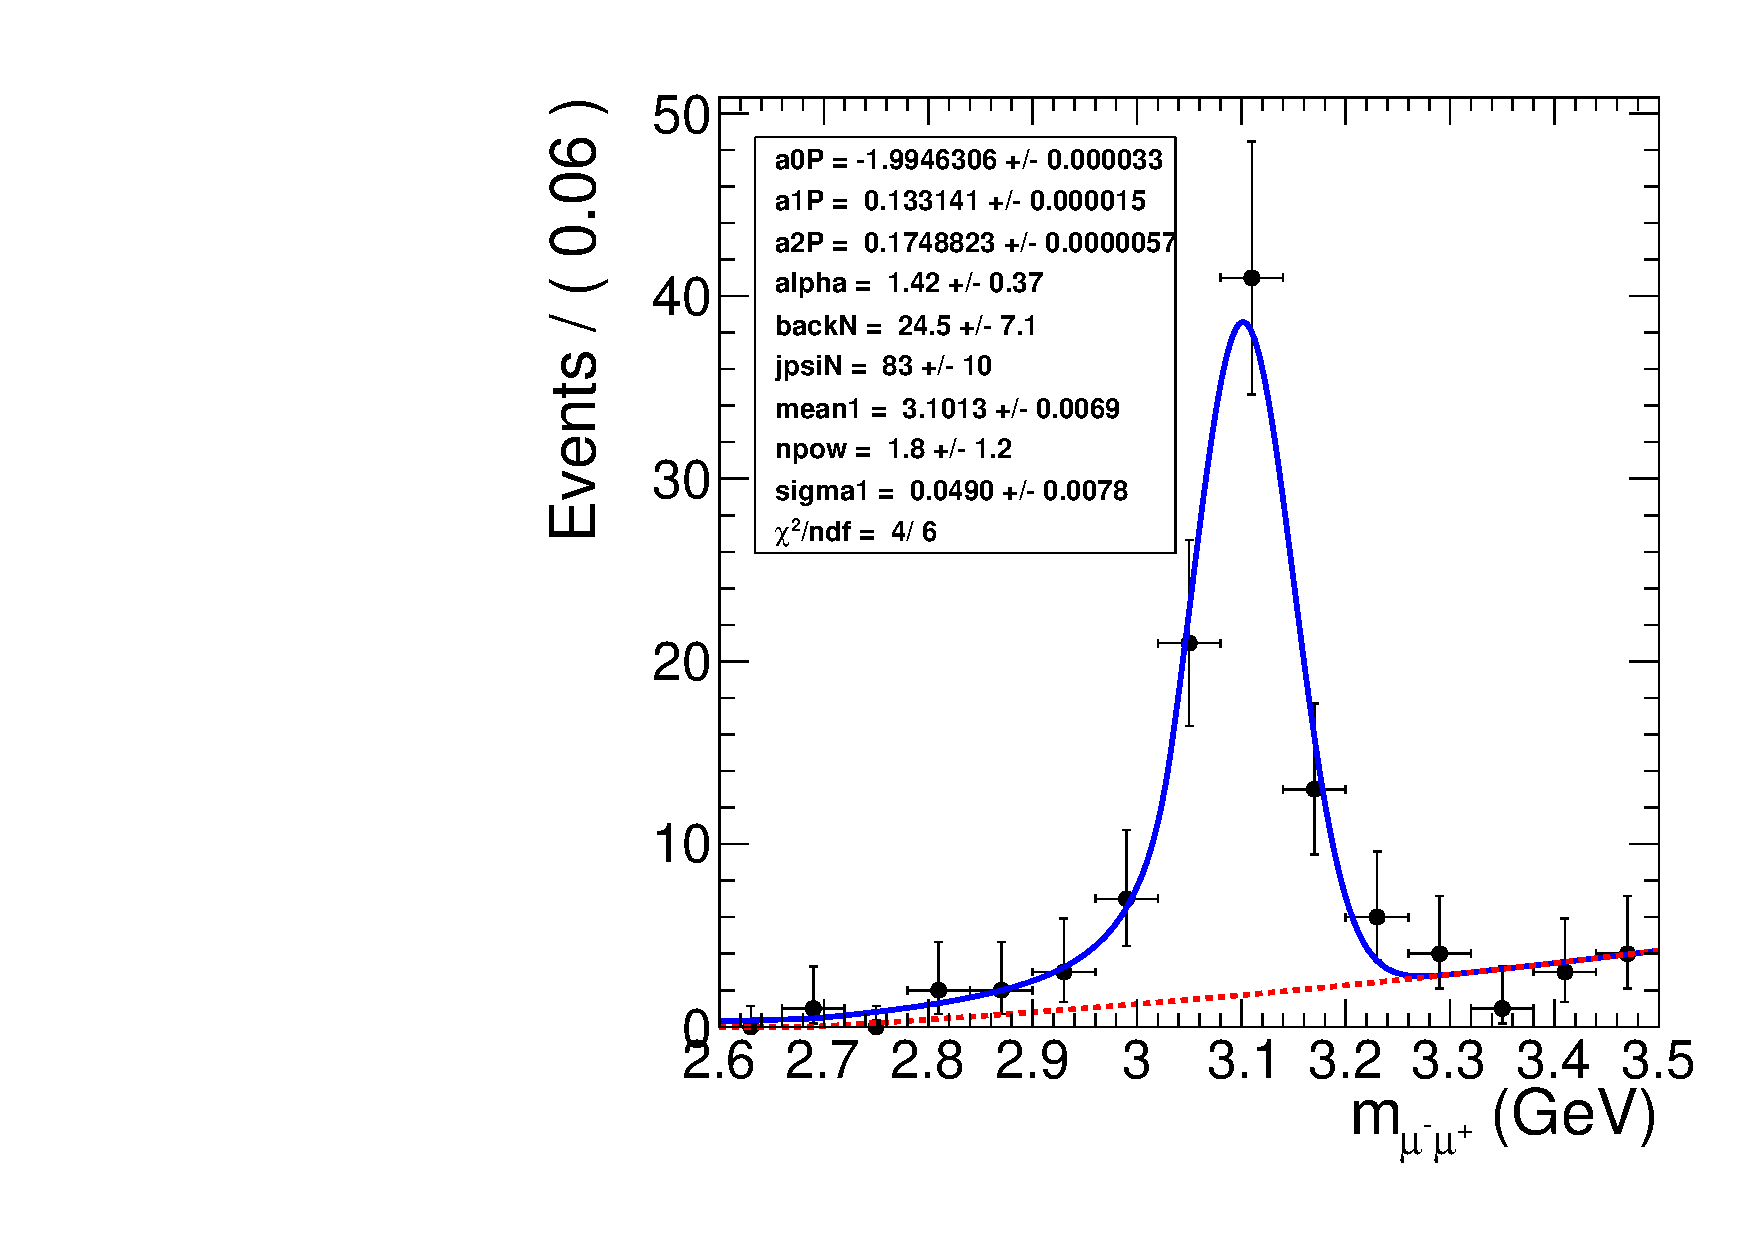
\includegraphics[width=.3\textwidth]{cbPolyBkgEst} &
        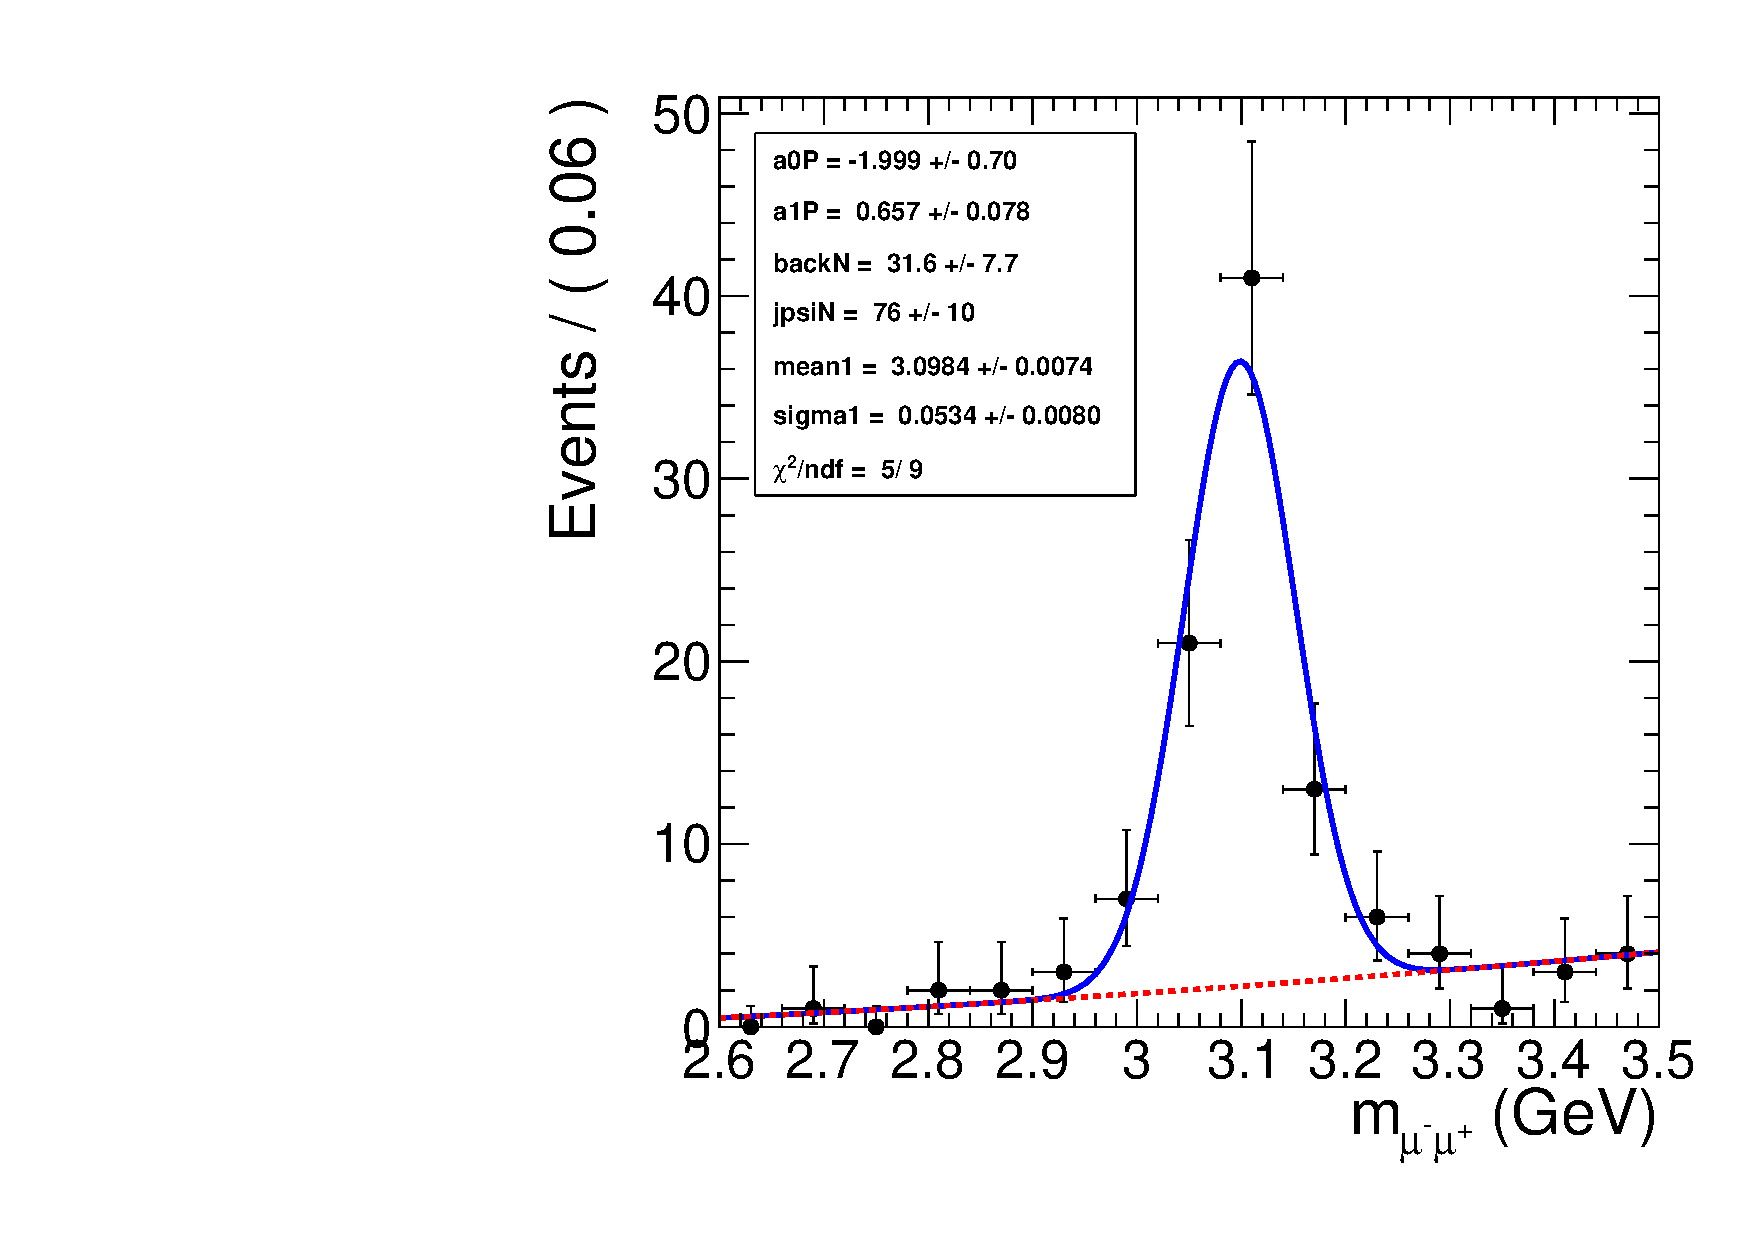
\includegraphics[width=.3\textwidth]{gausLinBkgEst} &
        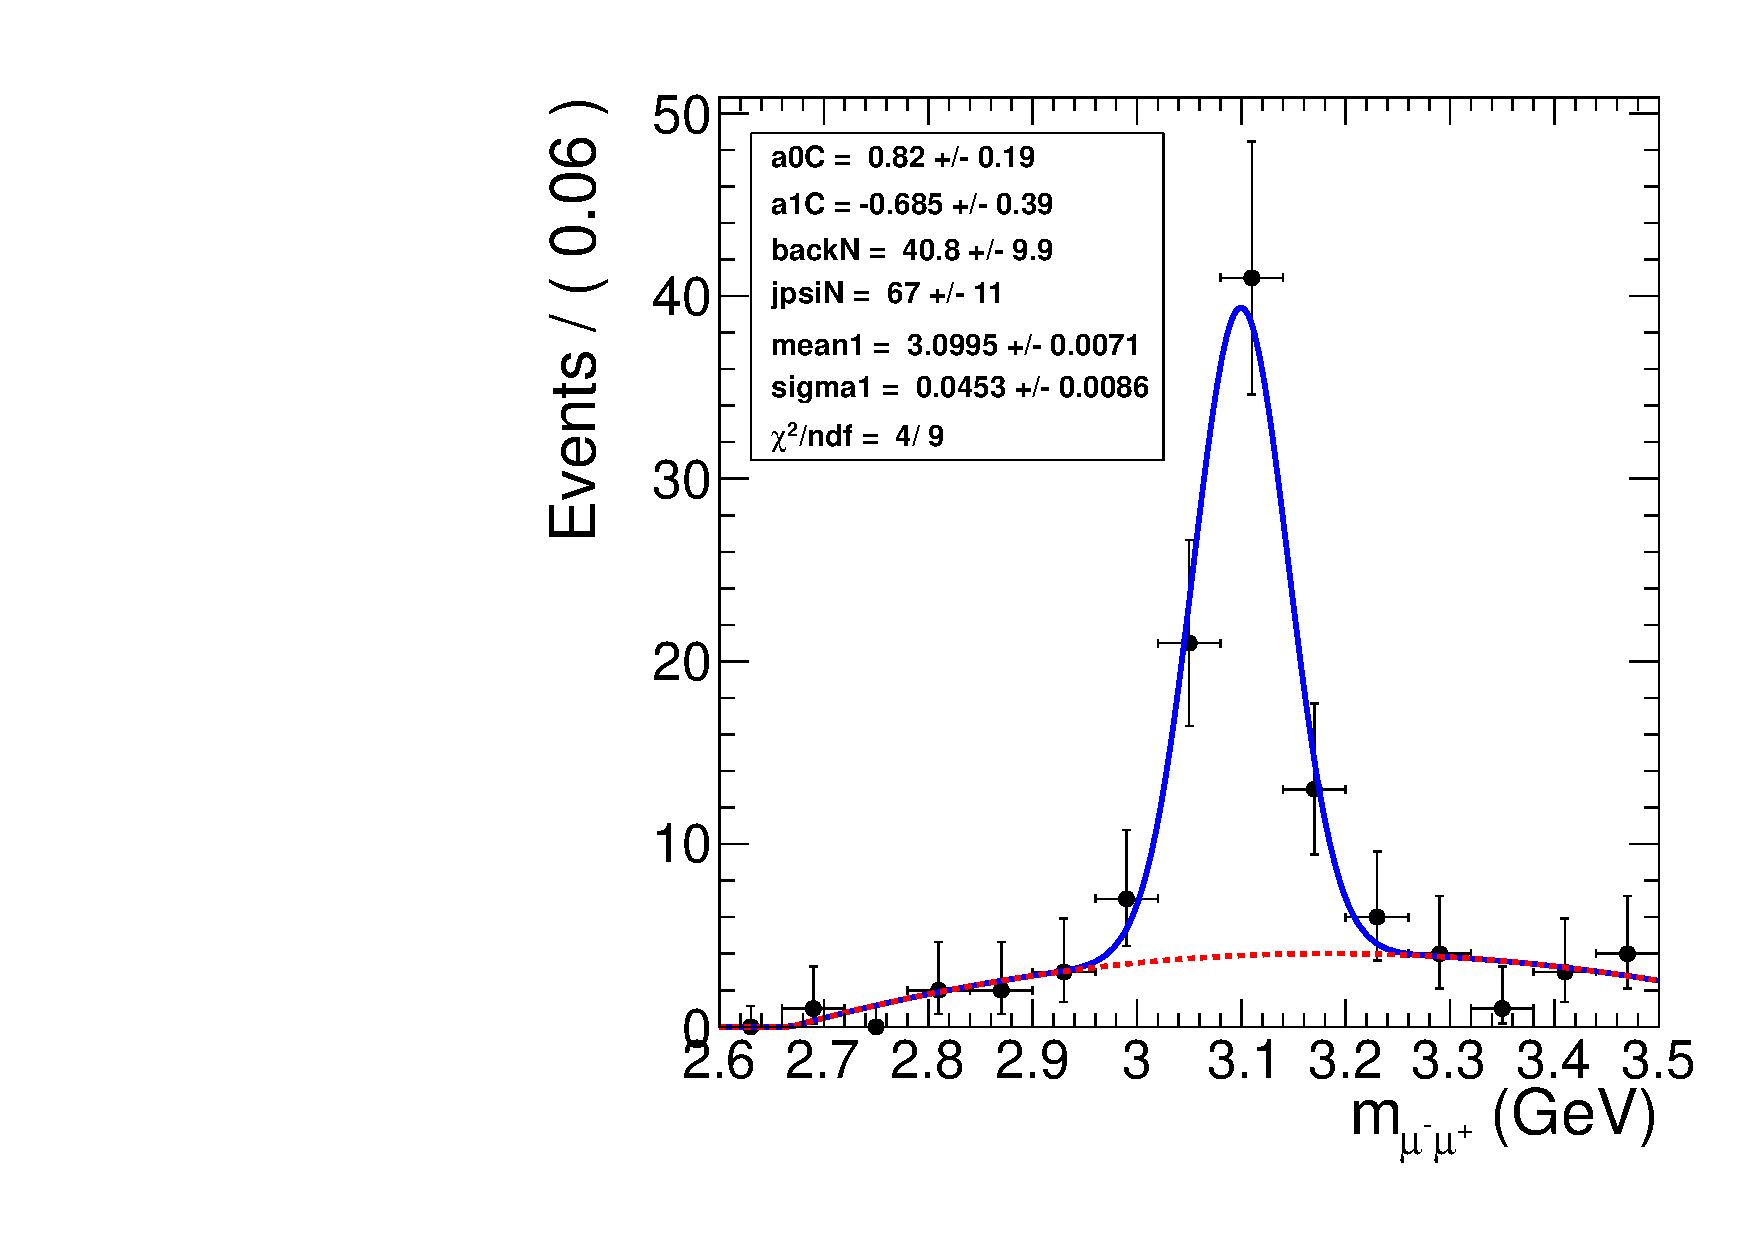
\includegraphics[width=.3\textwidth]{gausCCBkgEst} \\
        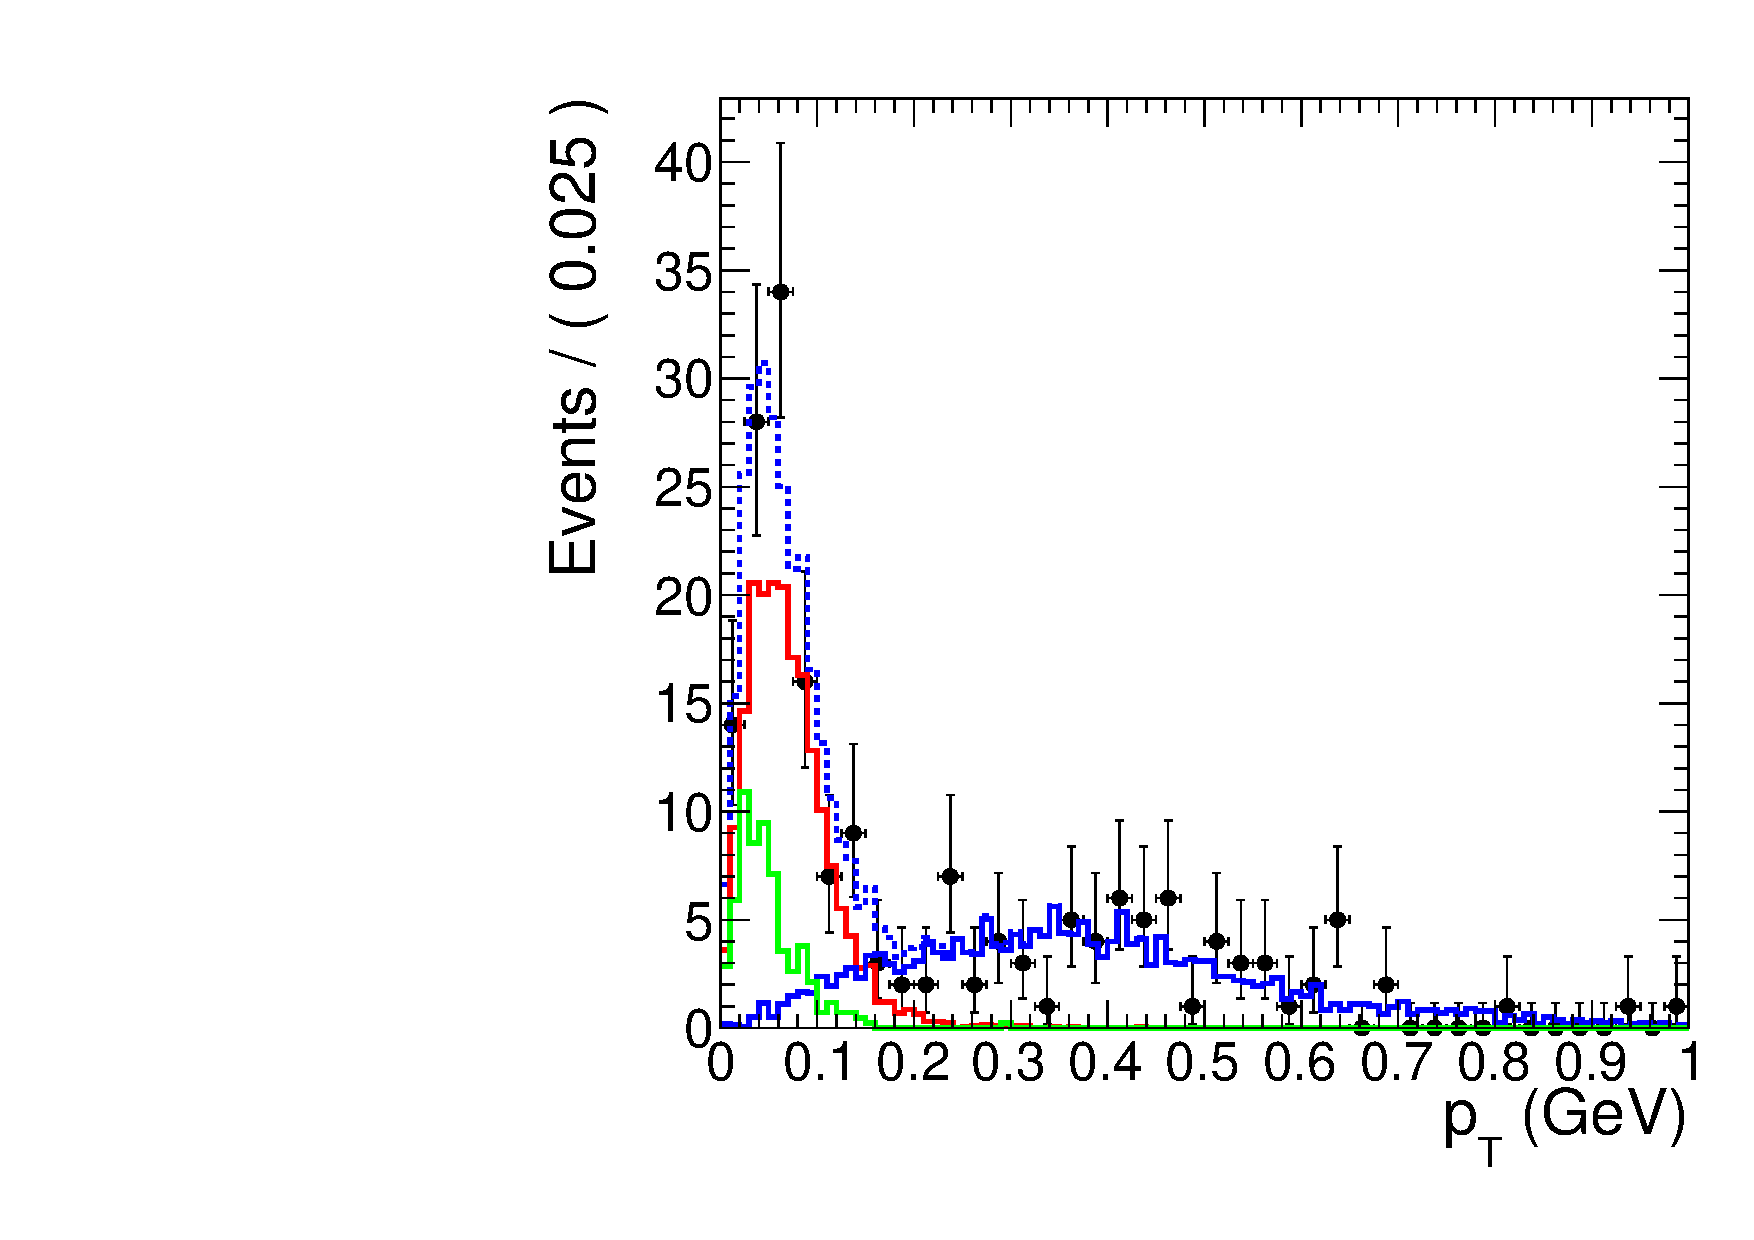
\includegraphics[width=.3\textwidth]{cbPoly} &
        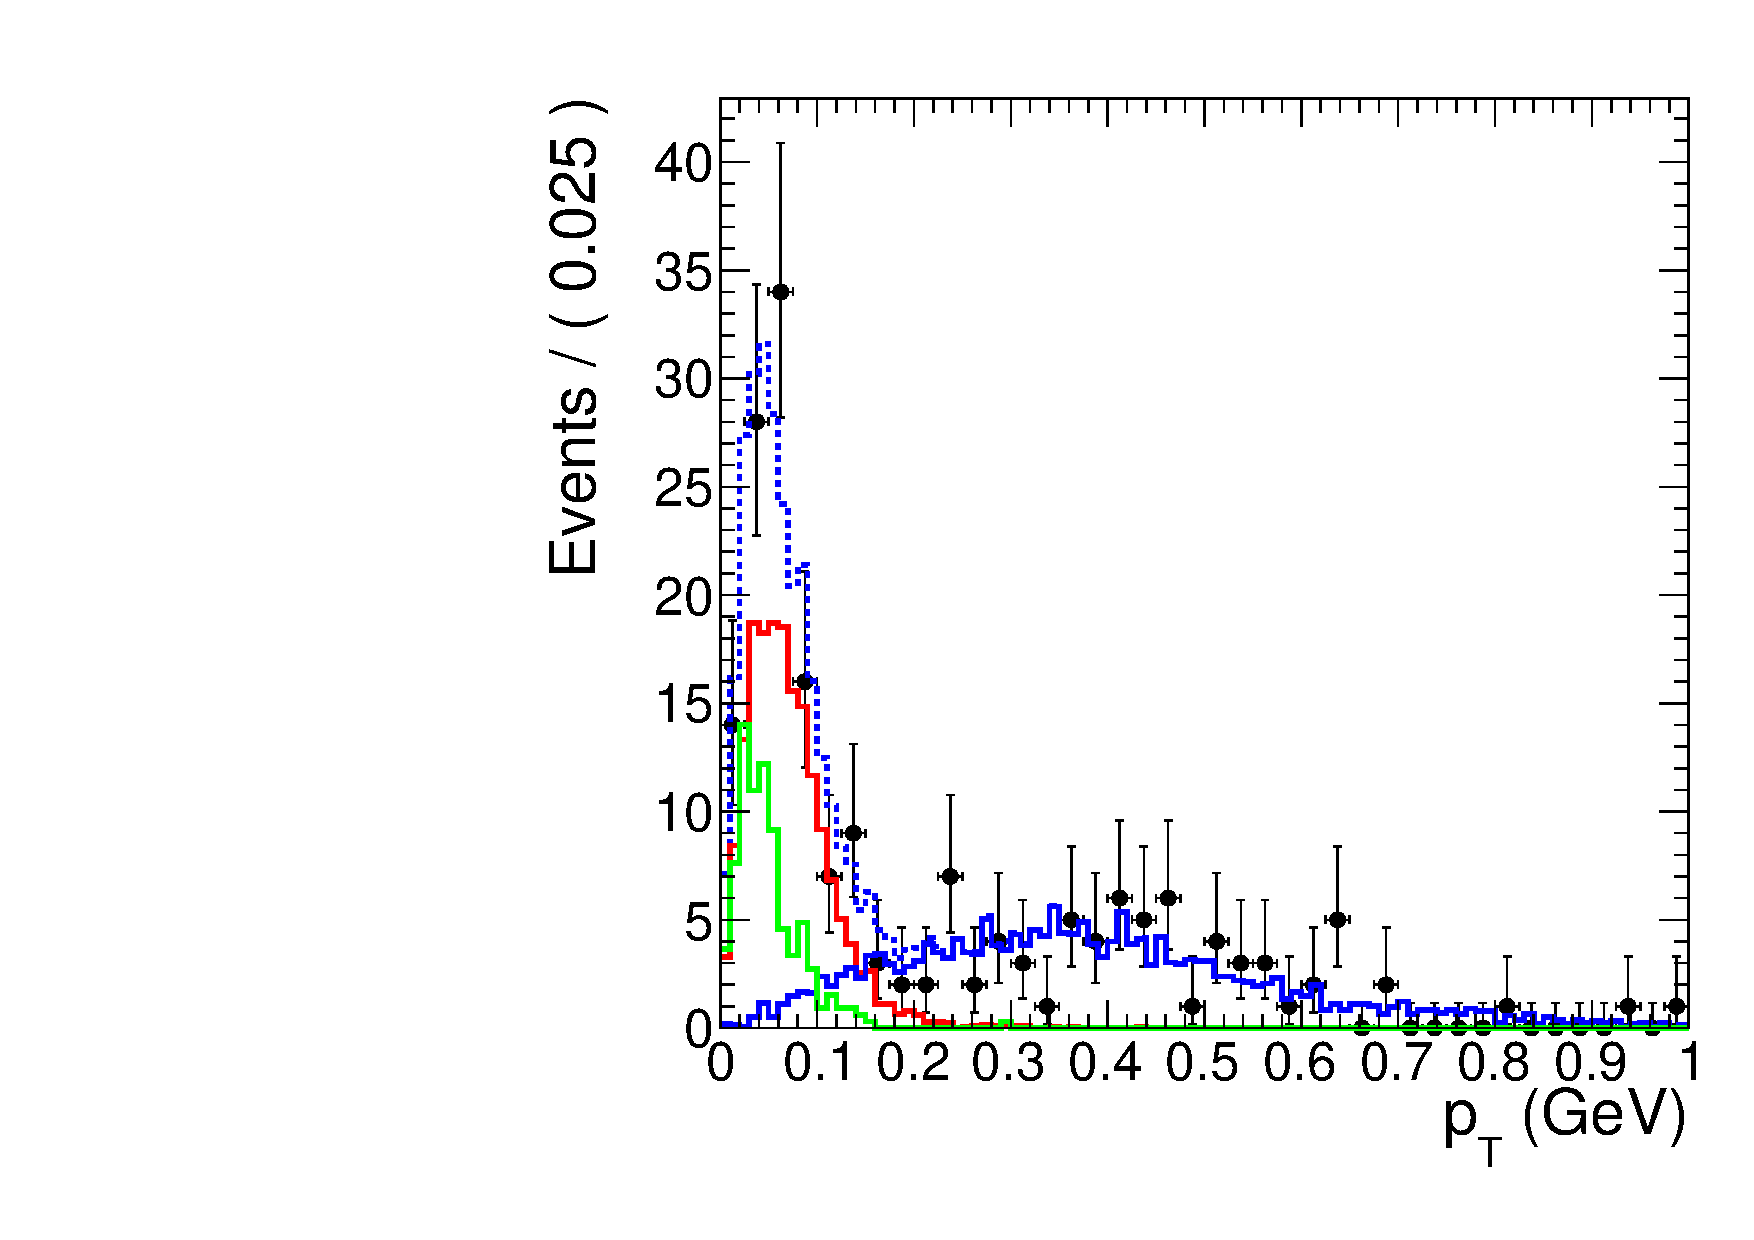
\includegraphics[width=.3\textwidth]{gausLin} &
        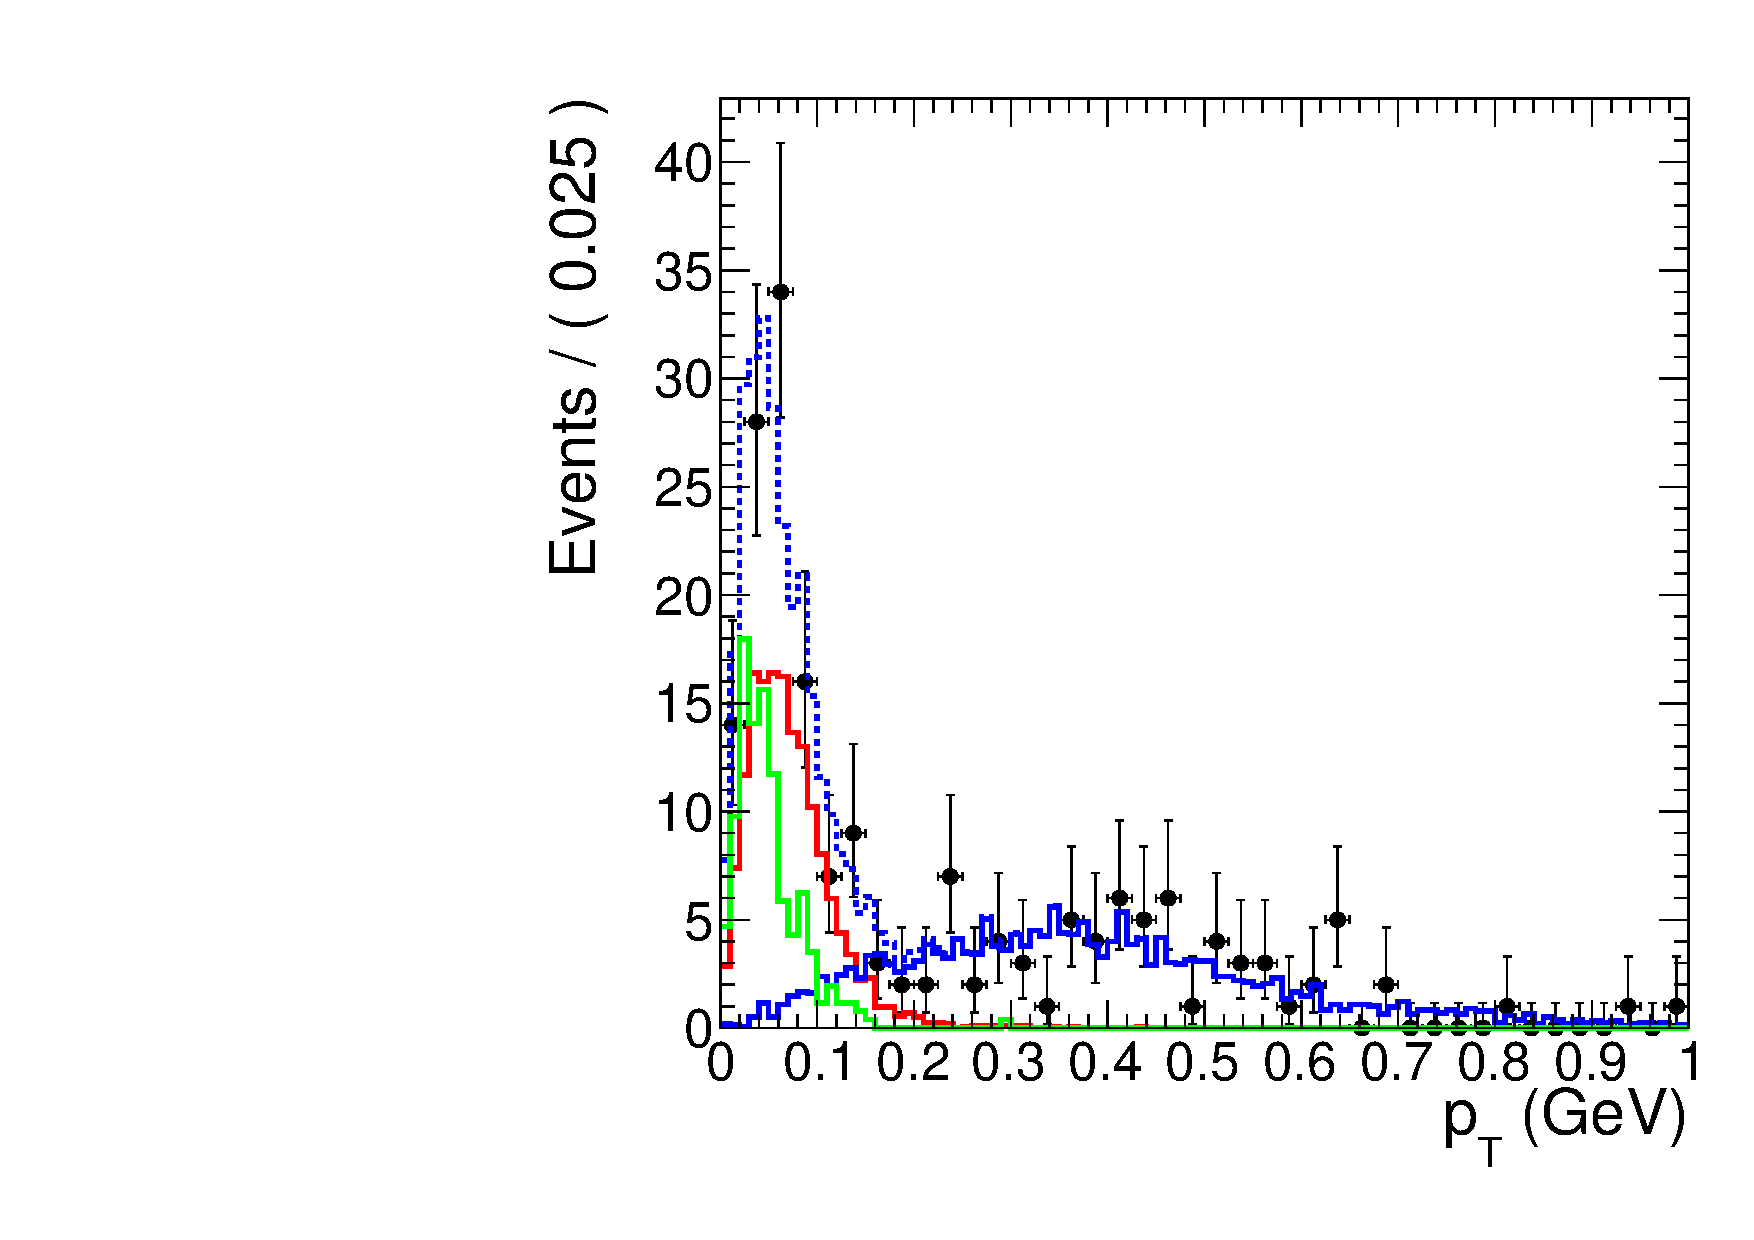
\includegraphics[width=.3\textwidth]{gausCC}
      \end{array} $
      \caption{Various mass distribution fits and the corresponding \pt{}
        template fit.}
      \label{fig:massPtFitsForSyst}
    \end{figure}

    Moving from left to right in Fig~\ref{fig:massPtFitsForSyst}, the 
      contribution from the photon-photon process increases.
    The $\chi^{2}$ / degree of freedom is similar between the three 
      fits indicating a similar goodness of fit.
    On this basis, neither fit is preferred. 
    The left most fit uses a Crystal Ball function to account for the 
      radiative decay of the final state daughters of the \JPsi{}.
    The low mass exponential portion however picks up background events 
      and overestimates the \JPsi{} contribution. 
    The right most plot fits the background to a 2nd order Cheby-Chev 
      polynomial.
    Because the Cheby-Chev peaks just below the \JPsi{} peak, this fit 
      overestimates the background and in turn underestimates the signal 
      contribution.
    The Gaussian fit with a linear background however does a reasonable job
      of fitting both the background and the signal. 

    From these three fits an upper and lower bound of the systematics due
      the choice of fit functions was estimated. 
    The difference between the Gaussian-Linear fit and the 
      Crystal Ball-polynomial fit was taken as an upper bound. 
    The difference between the Gaussian-Linear fit and the 
        Gaussian-Cheby-Chev fit was taken as a lower bound. 
    The overall systematic uncertainty due to the choose of normalization for
      the photon-photon template is found to be $^{+9.5\%}_{-12\%}$.

  \section{ZDC trigger efficiency}
    The ZDC trigger efficiency measurement is sensitive to the underlying 
      neutron distribution.
    The more neutrons that hit the ZDC, the higher the trigger efficiency 
      will be.
    To estimate the effect the input sample has on the efficiency, the ZDC 
      trigger efficiency was measured from five different samples.
    Table~\ref{tab:zdcEfficiencySys} shows the results from the 
      three samples, which require a reconstructed pixel track in the event to 
      reduce noise. 
    Both the nominal and alternative ZDC reconstruction methods are shown.
    \begin{table}
      \centering
      \begin{tabular}{|c|c|c|c|c|}
        \hline ZDC Side & Reco Method & N$_{events}$ & N$_{trig}$ & $\varepsilon_{ZDC}$ \\ \hline
         \multicolumn{5}{|c|}{(ZDC$^{+}$ or ZDC$^{-}$) and 1 pixel track} \\ \hline 
         ZDC$^{-}$ & alternative & 72946  & 71688 & 0.982 $\pm$ 0.005 \\ \hline
         ZDC$^{-}$ & nominal & 73028  & 71706  & 0.982  $\pm$ 0.005  \\ \hline
         ZDC$^{+}$ & alternative & 76137  & 71786  & 0.943  $\pm$ 0.005  \\ \hline
         ZDC$^{+}$ & nominal & 76132  & 71859  & 0.944  $\pm$ 0.005  \\ \hline
         \multicolumn{5}{|c|}{(ZDC$^{-}$ or ZDC$^{+}$), 1 pixel track, and L1 EG trigger } \\ \hline 
         ZDC$^{-}$ & alternative & 613758  & 602123  & 0.9810 $\pm$ 0.0018 \\ \hline
         ZDC$^{-}$ & nominal & 614014  & 601863  & 0.9802 $\pm$ 0.0018 \\ \hline
         ZDC$^{+}$ & alternative & 643905  & 602671  & 0.9360  $\pm$ 0.0017 \\ \hline
         ZDC$^{+}$ & nominal & 647888  & 603089  & 0.9309  $\pm$ 0.0017 \\ \hline
         \multicolumn{5}{|c|}{(ZDC$^{-}$ or ZDC$^{+}$), 1 pixel track, and L1 Muon trigger} \\ \hline 
         ZDC$^{-}$ & alternative & 65466  & 63376  & 0.968 $\pm$ 0.005  \\ \hline
         ZDC$^{-}$ & nominal & 65543  & 63358  & 0.967 $\pm$ 0.005 \\ \hline
         ZDC$^{+}$ & alternative & 71929  & 63512  & 0.883  $\pm$ 0.005 \\ \hline
         ZDC$^{+}$ & nominal & 72932  & 63582  & 0.872  $\pm$ 0.005 \\ \hline
       \end{tabular}
      \caption{ZDC trigger efficiencies using  the nominal and alternative 
        ZDC reconstructions for trigger sample that require a pixel track.}
      \label{tab:zdcEfficiencySys}
    \end{table}

    The systematic uncertainty in the ZDC trigger efficiency due to the 
      uncertainty in the underlying distribution was estimated by calculating 
      the standard deviation of efficiency measurements in Table~\ref{tab:zdcEfficiencySys}.
    The uncertainty in the ZDC trigger for ZDC$^{-}$ was found to be less than 
      1\% and taken to be negligible. 
    For ZDC$^{+}$, the systematic uncertainty was taken to be 3.5\%.

  \section{ZDC reconstruction}
    In order to estimated the systematic uncertainty in the ZDC reconstruction
      method, the alternative ZDC reconstruction method described in 
      Section~\ref{sec:zdcCompare} is used to measure the number of candidates
      in the Xn0n mode.
    The systematic uncertainty due to the ZDC reconstruction method is
      estimated from the difference between the UPC \JPsi{} candidate yields 
      when using the alternative versus the nominal method.
    The yields for the nominal and alternative ZDC reconstruction method in the 
      Xn0n break up were found to be 298 and 315 respectively. 
    Half the difference between the two methods was used as an estimate of 
      the systematic uncertainty, giving 2.9\%.

  \section{HF noise threshold}
    The way in which the HF noise distribution is measured effects the event 
      selection and therefore the final candidate yield.
    This cut plays a significant role in rejecting hadronic events.
    In Table~\ref{tab:evSelCutNumbers} the importance of cutting on HF noise
      is evident. 
    The HF noise cut rejects nearly 1/5 of the remaining events. 
    The systematic uncertainties on the HF noise requirement is important for
      this reason.
   
    The most basic information from the HF detectors are contained in RecHits. 
    There is one RecHit per phototube on HF. 
    The RecHit signal is calibrated in GeV, and no noise subtraction is done. 
    The CaloTowers are formed from geometrical groups of RecHits. 
    They are the first stage of the CMS jet trigger and perform some noise 
      suppression.

    The default HF noise cut required that the maximum RecHit energy
      from both HF+ and HF- be less than 3.85 GeV. 
    This cut was designed to accept 99\% of the noise events, 
      see Fig.~\ref{fig:hfNoiseDist}. 
    The stability of this cut was tested by
    \begin{enumerate}
      \item Summing CaloTowers instead of RecHits
      \item Making separate cuts on HF- and HF+
      \item Tightening the threshold so that only 98\% or 97\% noise events 
        passed the cut.
    \end{enumerate}
    \begin{table}[!Hhbt]
      \centering
      \begin{tabular}{|c|c|c|c|}
        \hline
        Object type & HF (GeV) & HF$^{-}$ (GeV) & HF$^{+}$ (GeV) \\ \hline
        RecHits & 3.85 & 3.25 & 3.45 \\ \hline
        CaloTowers & 4.25 & 3.25 & 3.75 \\ \hline
      \end{tabular}
      \caption{Thresholds from combined HF noise distributions and 
        two-side noise distributions.}
      \label{tab:hfNoiseThreshAsym}
    \end{table}

    \begin{table}[!Hhbt]
      \centering
        \begin{tabular}{|c|c|c|} \hline
          \% &  $E_{RecHit}$ (GeV) & $E_{CaloTower}$ (GeV)\\ 
          \hline
          99 & 3.85& 4.25 \\ \hline
          98 & 3.25& 3.75 \\ \hline
          97 & 2.95& 3.25 \\  \hline
         \end{tabular}
        \caption{HF noise thresholds for keeping various fractions of the noise
          sample for RecHit and CaloTower.}
        \label{tab:hfAdjustedThresholds}
    \end{table}

    Table~\ref{tab:hfNoiseThreshAsym} shows the noise thresholds for RecHits 
      and CaloTowers for both the combined HF+ and HF- calorimeters and the 
      two-sided individual calorimeters when 99\% of noise events are accepted.
    Table~\ref{tab:hfAdjustedThresholds} compares the threshold for the cases 
      when 99\%, 98\% and 97\% of noise events are accepted.
    The number of \JPsi{} events remaining after these cuts is shown in 
      Table~\ref{tab:hfAdjThreshYields}. 
    The efficiency corrected numbers are also shown in order to compare between
      different noise thresholds. 
    The fractional systematic error is then estimated by finding the maximum 
      and minimum deviation from the default method. 
    The nominal number of candidates come from the 99\% combined RecHit 
      threshold.
    From Table~\ref{tab:hfAdjThreshYields}, the maximum number of corrected 
      candidates comes from the 99\% threshold for combined CaloTower objects,
      and the minimum from 97\% threshold for the same objects. 
    The fractional increase from the maximum of 305 corrected candidates and 
      the nominal value of 301 is taken as the systematic upper bound; the 
      bound is estimated from the minimum of 289, giving a systematic 
      uncertainty of $^{+0.3\%}_{-3.4\%}$.
    \begin{table}[!Hhbt]
      \centering
        \begin{tabular}{|c|c|c|c|c|c|} \hline
          \% &  RecHit cut & RecHit corrected & CaloTower cut & CaloTower corrected & Threshold type \\ \hline
          99 & 298 & 301 & 302 & 305 & \multirow{3}{*}{Combined} \\ \hhline{-----~}
          98 & 287 & 293 & 294 & 300 & \\ \hhline{-----~}
          97 & 284 & 292 & 280 & 289 & \\ \hline \hline
          99 & 290 & 293 & 288 & 291 & Two-sided \\ \hline
        \end{tabular}
      \caption{Number of upc dimuon candidates with  p$_{T} <$ 1 GeV when changing HF calorimeter cuts for RecHit and CaloTower.}
      \label{tab:hfAdjThreshYields}
    \end{table}

  \section{MC acceptance}
    The MC derived acceptance correction factors depend on the input physics
      generator. 
    The underlying \pt{} distribution was assumed to be correctly 
      described by STARlight for the coherent cross section measurement.
    To estimate the effect of changing the underlying \pt{} distribution 
      on the acceptance measured from the MC, the incoherent sample was used 
      to correct the coherent yield.
    Half the difference was used as the estimate and was found to be 1.1\%.

  \section{\label{sec:extraSys}Additional cross checks}
    \subsection{Simultaneous fit using mass templates}
      As check on the simultaneous \pt{} and mass fit, the mass fit is done
        using mass templates from STARlight.
      The coherent fraction, $f_{co}$, using the mass template for the 
        simultaneous fit gave 0.60 $\pm$ 0.09, which is consistent with the 
        nominal method described in Section~\ref{sec:sigEx}.
      \begin{figure}[!Hhbt]
        \centering
        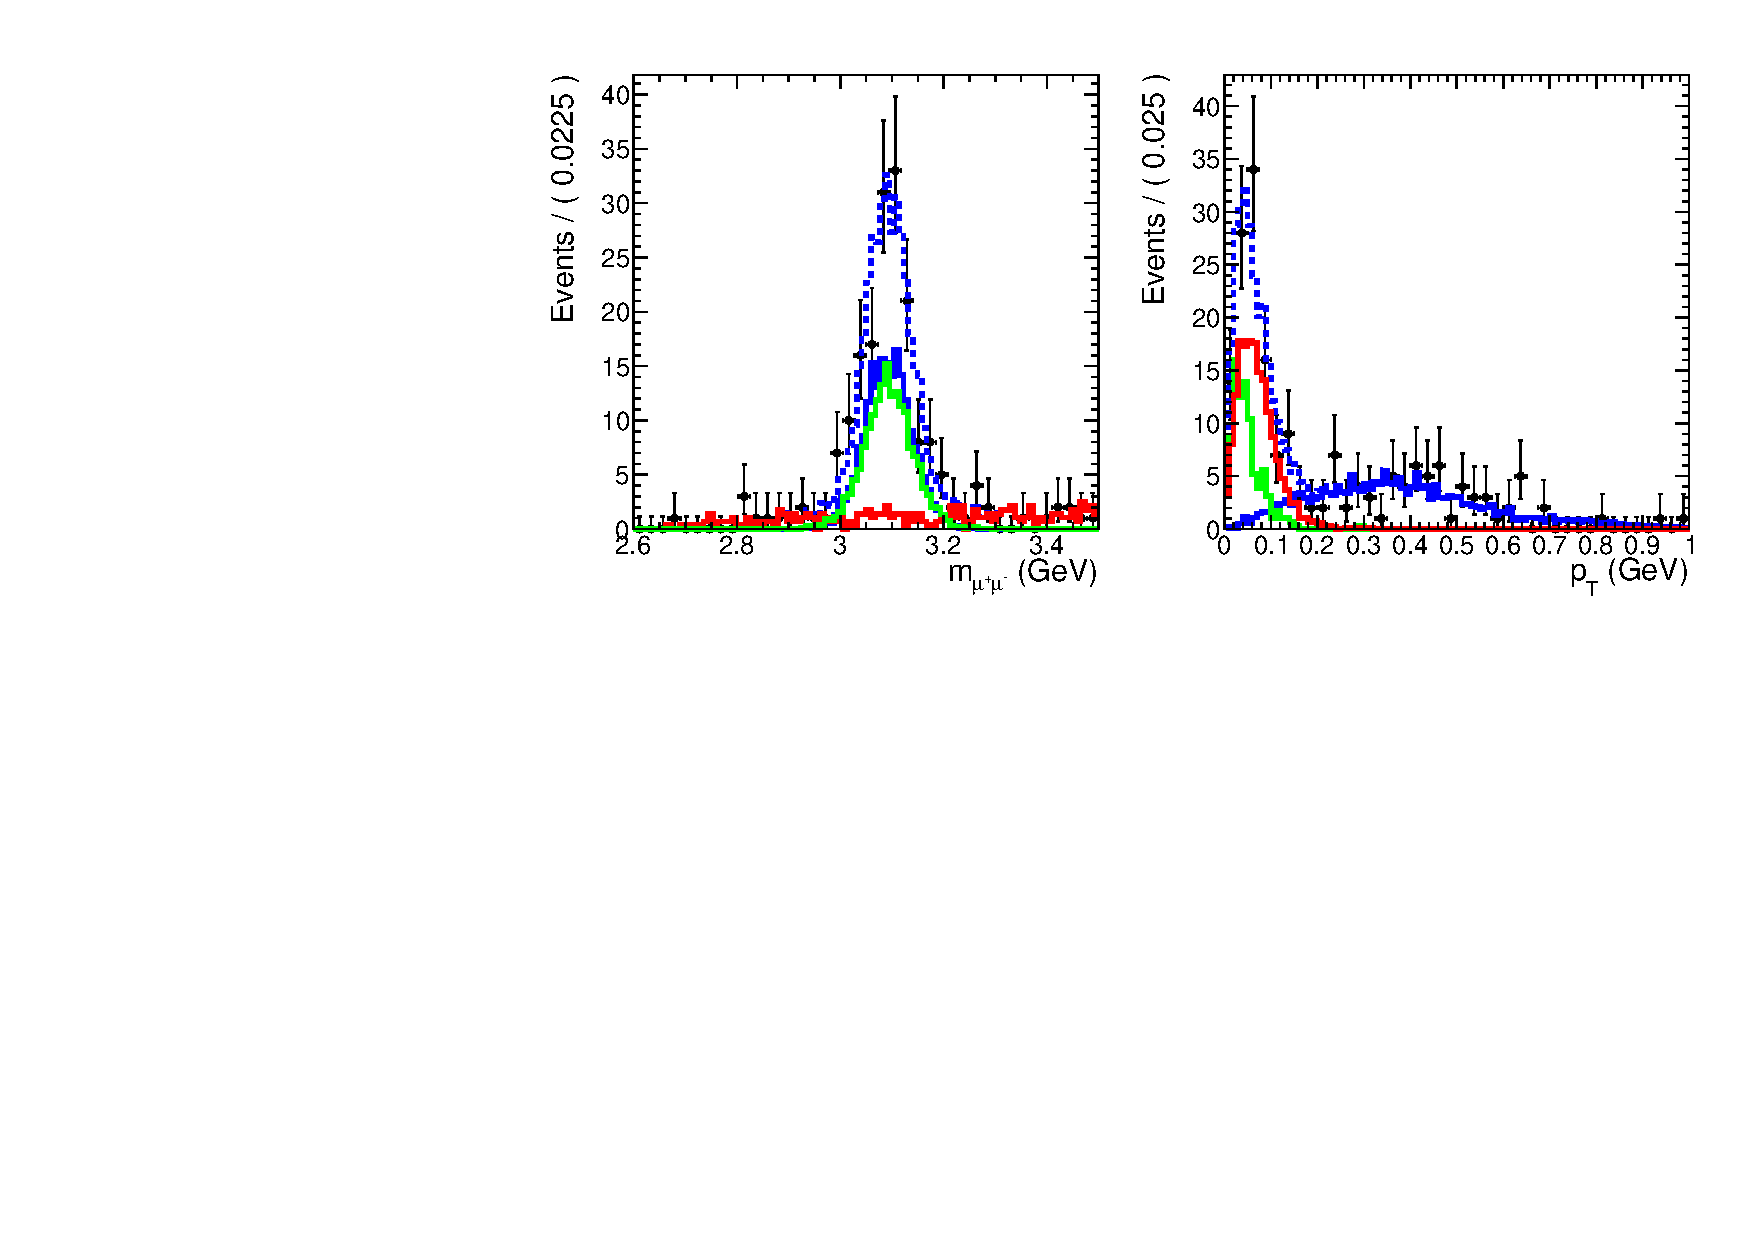
\includegraphics[width=0.6\textwidth]{ptMassSimTemp}
        \caption{Simultaneous fit to the mass and \pt{} using mass templates
          for the mass fit. }
        \label{fig:simFitTemp}
      \end{figure}
  
    \subsection{Tag and probe from counting compared to fitting}
      The main purpose for fitting the mass spectra to estimate the efficiency
        is to separate the background from true signal. 
      The background may not have the same efficiency as the signal, so 
        separating the two is important if this is the case.
      In the tag and probe fit the signal peak from the \JPsi{} resonance
        is fit to the probes, passing probes, and failing probes alike (see
        Fig.~\ref{fig:tnpFitPlot}). 
      The signal shape, if from the same physical signal, will be 
        identical in each of the three distributions. 
      The background for the passing and failing probes is fit using 
        different parameters for the background because the background
        may come from different physical processes than the signal, or from 
        non-physical sources like combinatorial backgrounds or misidentified
        fake particles.
      When the background comes from sources other than the physical signal,
        the background may give an efficiency estimate that is lower than
        the signal. 
  
      The trigger efficiency measured by the tag and probe method depends on
        the fitting functions use to estimate the background and signal 
        contributions. 
      Depending on what functions is used to fit the spectra, the amount of
        background can be over or underestimated and effect the efficiency 
        measurement.
      To estimate this effect, the tag and probe efficiencies were additionally
        measured by counting probes in the \JPsi{} mass window. 
      The whole mass window is used to estimate the efficiency including all 
        the events from the mass side bands.
      In this way, a worst case scenario estimate is given where all background
        events are included as signal. 
      \begin{figure}[!Hhbt]
        \centering
        $ \begin{array}{cc}
          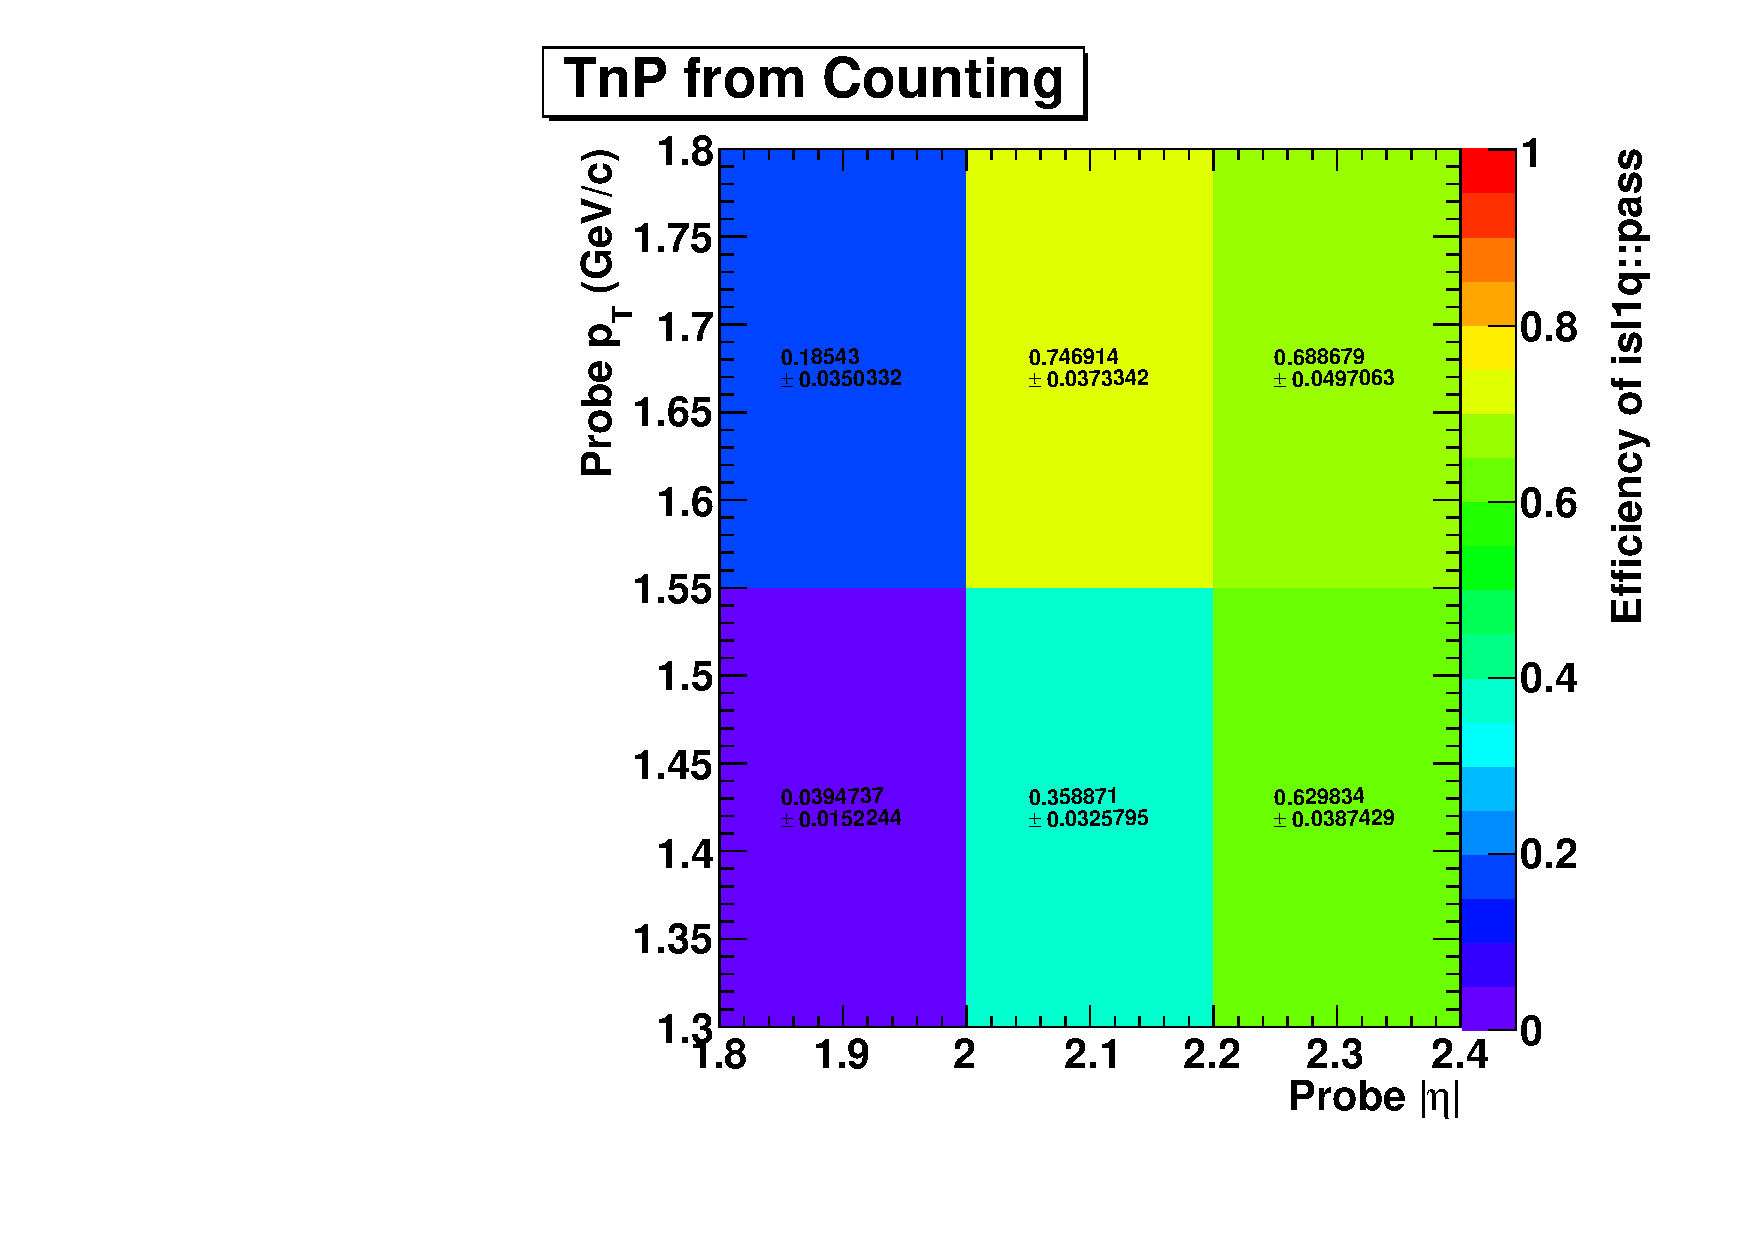
\includegraphics[width=.45\textwidth]{tNp/tnpFromCounting} &
          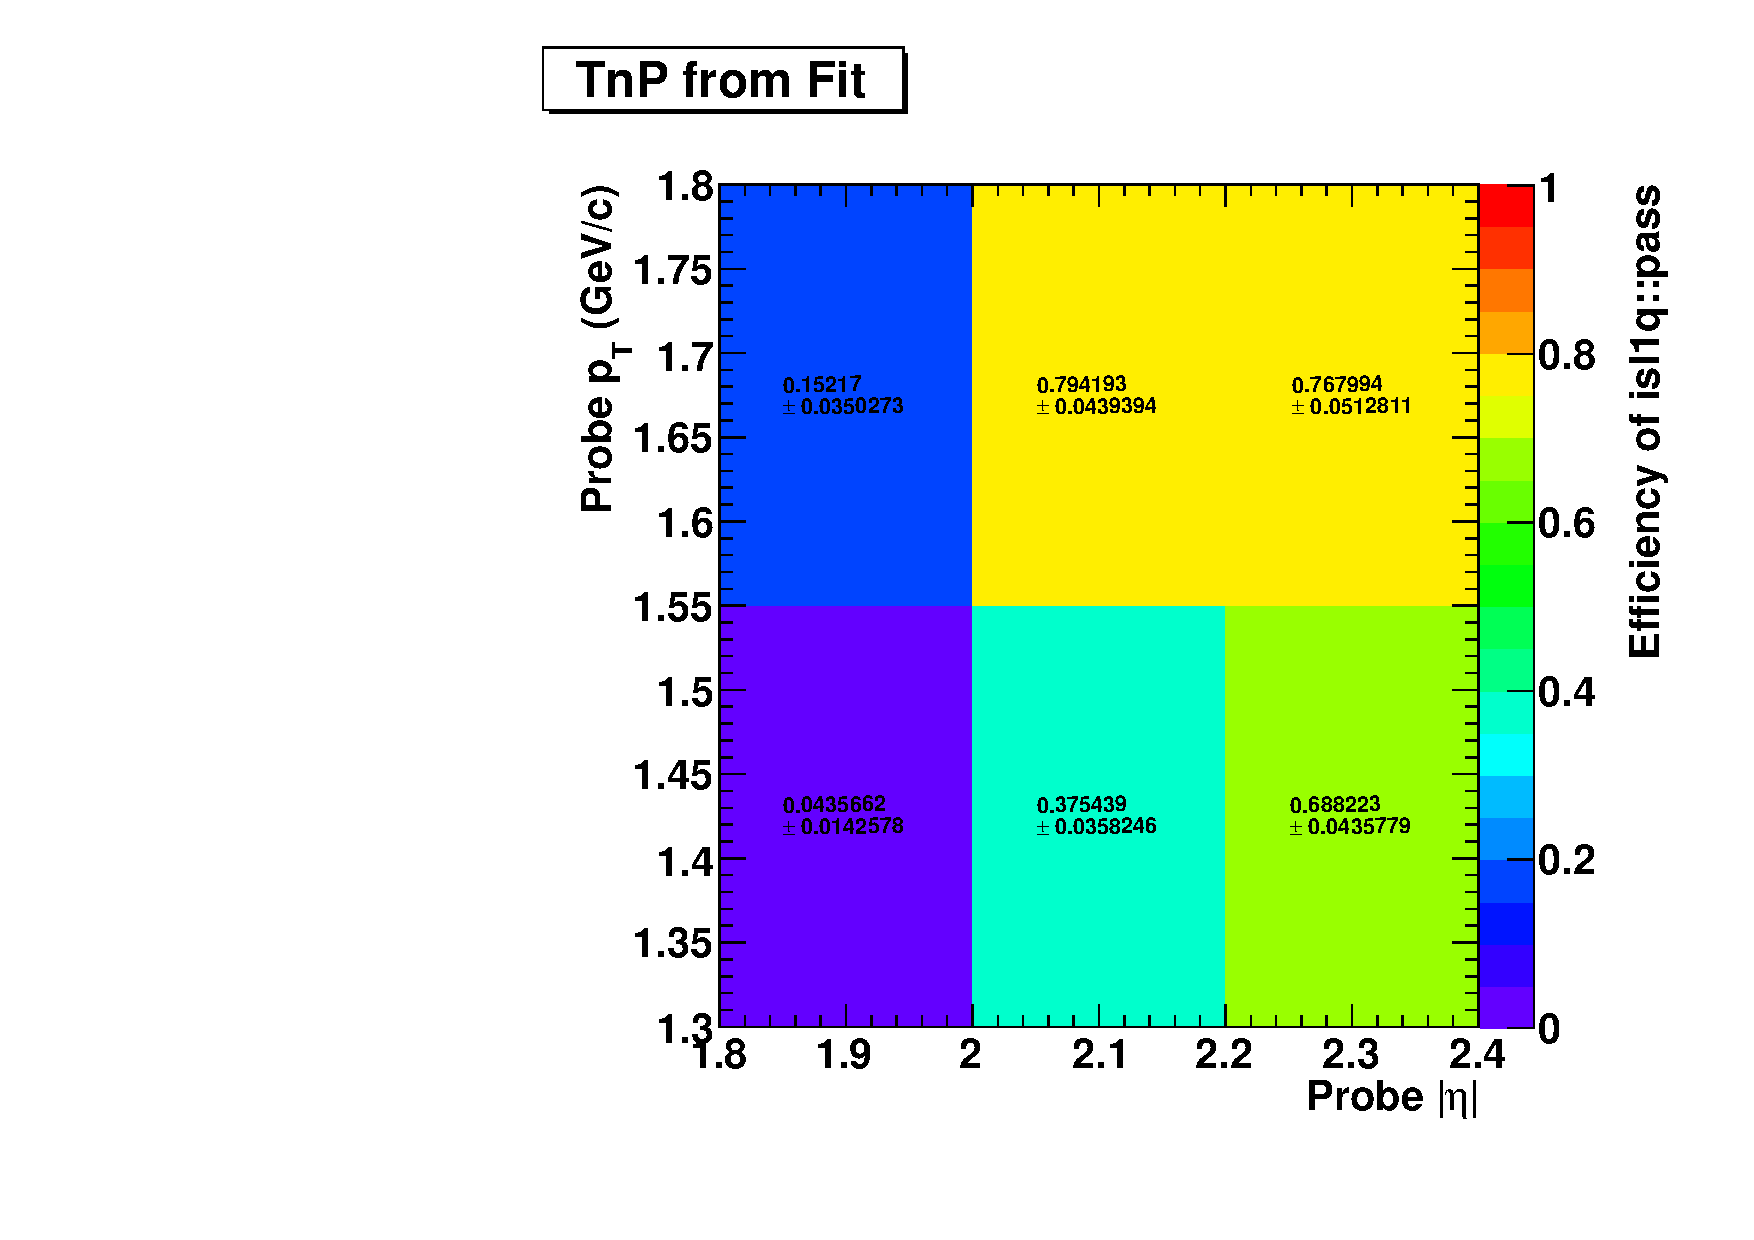
\includegraphics[width=.45\textwidth]{tNp/tnpFromFit}
        \end{array} $ 
        \caption{Tag and probe trigger efficiencies from counting (left) 
          compared to fitting (right).}
        \label{fig:tnpCntVFit}
      \end{figure}
  
      From Fig.~\ref{fig:tnpCntVFit} it is apparent that the choice of fit 
        function, and, therefore, the amount of background from the mass side 
        bands is included in the signal measurement has very little effect on 
        the tag and probe efficiency measurement.
      For example for muons with $\eta$ between 2.0 and 2.2 and \pt{} between
        1.50 GeV and 1.75 GeV the counting method gives a trigger efficiency 
        of $0.764 \pm 0.034$ compared to $0.794 \pm 0.044$ for the fitting 
        method. 
      The small effect of including the side bands are due to the side bands 
        being comprised mostly of photon-photon events.
      Because this background is neither decays from other particles like pions,
        nor is it from non-physical background like combinatorics, 
        the efficiency for muons from the side bands are nearly identical to
        \JPsi{} signal.
      The photon-photon process directly produces two muons just like the 
        \JPsi{}, therefore efficiency estimated from the side bands has 
        little effect on the measurement because of this similarity.
      The counting and fitting trigger efficiency measurements agree within 
        statistical uncertainties, so this uncertainty was taken to be 
        negligible.
  
    \subsection{The effect of noise on ZDC trigger efficiency estimates}
      The amount of electronic noise in the sample effects the ZDC energy 
        distribution and, therefore, the trigger efficiency measurement.
      The more noise that sits below the one neutron peak, the lower the 
        efficiency estimate will be. 
      In Table~\ref{tab:zdcEfficiencySysNoiseSample}, the zero bias sample 
        with the timing cuts desribed in Section~\ref{sec:zdcCompare} gives a 
        significantly higher
        estimated efficiency compared the zero bias sample with out timing cuts
        in Table~\ref{tab:zdcEfficiencySysNoiseSample}.
      The same increase is seen when comparing the ZDC triggered sample with 
        the ZDC triggered sample that also requires a pixel track shown in
        Table~\ref{tab:zdcEfficiencySys}. 
      The effect of the electronic noise is also present in the difference seen
        in using the two methods.
      As seen in Fig.~\ref{fig:zdcSpec2v1}, the new reconstruction method 
        shows better separation of the one neutron peak from the electronic 
        noise, in particular in ZDC$^{+}$ where the signal gain is lower.
      For this reason, the zero bias data, which contains the largest 
        contribution from electronic noise, shows the most separation between 
        the two methods and gives the lowest estimate for the ZDC trigger 
        efficiency.
      \begin{table}
        \centering
        \begin{tabular}{|c|c|c|c|c|}
          \hline ZDC Side & Reco Method & N$_{events}$ & N$_{trig}$ & $\varepsilon_{ZDC}$ \\ \hline
          \multicolumn{5}{|c|}{ Zero bias with ZDC timing cuts} \\ \hline 
           ZDC$^{-}$ & alternative & 88676  & 84429  & 0.9521 $\pm$ 0.0046 \\ \hline
           ZDC$^{-}$ & nominal & 88480  & 84202  & 0.9517 $\pm$ 0.0046 \\ \hline
           ZDC$^{+}$ & alternative & 59878  & 54728  & 0.9140  $\pm$ 0.0054 \\ \hline
           ZDC$^{+}$ & nominal & 60467  & 54733  & 0.9052  $\pm$ 0.0053 \\ \hline
           \multicolumn{5}{|c|}{(ZDC$^{-}$ or ZDC$^{+}$)} \\ \hline 
           ZDC$^{-}$ & alternative & 30986 & 30333 & 0.9789 $\pm$ 0.0079 \\ \hline
           ZDC$^{-}$ & nominal & 31029 & 30339 & 0.9778 $\pm$ 0.0079 \\ \hline
           ZDC$^{+}$ & alternative & 39178 & 30164 & 0.7699 $\pm$ 0.0059 \\ \hline
           ZDC$^{+}$ & nominal & 35703 & 30443 & 0.8527 $\pm$ 0.0067 \\ \hline
           \multicolumn{5}{|c|}{ Zero bias} \\ \hline 
           ZDC$^{-}$ & alternative & 109967  & 101598  & 0.9239 $\pm$ 0.0040 \\ \hline
           ZDC$^{-}$ & nominal & 110230  & 101561  & 0.9214 $\pm$ 0.0040 \\ \hline
           ZDC$^{+}$ & alternative & 253241  & 86660  & 0.3422 $\pm$ 0.0013 \\ \hline
           ZDC$^{+}$ & nominal & 156336  & 87401  & 0.5591 $\pm$ 0.0024 \\ \hline
         \end{tabular}
        \caption{ZDC trigger efficiencies using  the nominal and alternative 
        ZDC reconstructions for trigger sample that do no require a pixel track.}
        \label{tab:zdcEfficiencySysNoiseSample}
      \end{table}
